\chapter{Vectorized Streaming Data Pipeline \& Systems Engineering}
\label{ch:data_pipeline}

\section{Introduction and High-Velocity Ingestion Challenges}
Financial transaction networks generate massive streaming volumes, requiring ingestion engines to process hundreds of thousands of events per second while maintaining strict temporal causality, dynamic schema flexibility, and sub-millisecond query latencies. Traditional relational databases (e.g., PostgreSQL) or distributed frameworks (e.g., Apache Spark) introduce severe serialization overheads, disk I/O bottlenecks, and network round-trip latencies that violate payment authorization service-level agreements (SLAs).

To resolve these challenges, C-STGB incorporates a vectorized, zero-copy streaming ingestion engine built on embedded DuckDB, Apache Arrow in-memory columnar buffers, and Least Recently Used (LRU) topological subgraph caches.

\begin{figure}[htbp]
\centering

\includegraphics[width=\textwidth]{figures/fig_canonical_invariants.pdf}
\caption{Vectorized streaming data engineering architecture, illustrating zero-copy Arrow ingestion, DuckDB SQL data contracts, dynamic schema discovery, and in-memory LRU causal subgraph caching.}
\label{fig:ch4_pipeline_architecture}
\end{figure}

\section{DuckDB Embedded Analytical Engine \& SQL Data Contracts}
C-STGB deploys DuckDB as an in-process, columnar analytical execution engine. By operating entirely within the same memory address space as PyTorch Geometric, DuckDB eliminates inter-process communication (IPC) serialization penalties.

\subsection{Standardized Transaction SQL Data Contract}
\label{lst:duckdb_schema}\label{lst:duckdb_entities}
Every incoming financial transaction payload and reference entity must strictly adhere to the unified streaming relational data contracts formalized in Listings~\ref{lst:duckdb_schema} and~\ref{lst:duckdb_entities}.

\begin{small}
\begin{verbatim}
CREATE TABLE streaming_transactions (
    transaction_id VARCHAR(64) PRIMARY KEY,
    source_entity_id VARCHAR(64) NOT NULL,
    target_entity_id VARCHAR(64) NOT NULL,
    timestamp_epoch DOUBLE NOT NULL,
    amount_raw DOUBLE NOT NULL,
    amount_usd DOUBLE NOT NULL,
    currency_code VARCHAR(8) NOT NULL,
    channel_type VARCHAR(16) NOT NULL,
    fee_amount DOUBLE DEFAULT 0.0,
    is_sar_alert BOOLEAN DEFAULT FALSE,
    ingest_timestamp TIMESTAMP DEFAULT CURRENT_TIMESTAMP
);

CREATE INDEX idx_source_time ON streaming_transactions (source_entity_id, timestamp_epoch);
CREATE INDEX idx_target_time ON streaming_transactions (target_entity_id, timestamp_epoch);

CREATE TABLE entities_master (
    entity_id VARCHAR(64) PRIMARY KEY,
    entity_type VARCHAR(32) NOT NULL, -- 'individual', 'merchant', 'financial_institution', 'smart_contract'
    country_iso VARCHAR(3) NOT NULL,
    kyc_risk_tier INTEGER DEFAULT 1,  -- 1 (Low) to 5 (Critical)
    is_pep BOOLEAN DEFAULT FALSE,     -- Politically Exposed Person
    is_sanctioned BOOLEAN DEFAULT FALSE,
    registration_timestamp TIMESTAMP NOT NULL,
    last_active_timestamp TIMESTAMP NOT NULL
);

CREATE TABLE high_risk_jurisdictions (
    country_iso VARCHAR(3) PRIMARY KEY,
    fatf_status VARCHAR(16) NOT NULL, -- 'black_list', 'grey_list', 'standard'
    basel_aml_index DOUBLE NOT NULL,
    sanction_regime VARCHAR(64) DEFAULT 'None'
);
\end{verbatim}
\end{small}

\subsection{Causal Ego-Graph Analytical Query Execution}
To extract the localized $k$-hop causal ego-graph $\mathcal{N}_k(u, t)$ strictly prior to transaction timestamp $t$, DuckDB executes vectorized columnar filtering:
\begin{small}
\begin{verbatim}
SELECT 
    t.source_entity_id,
    t.target_entity_id,
    t.amount_usd,
    t.timestamp_epoch,
    ( ? - t.timestamp_epoch ) AS delta_time,
    e_src.kyc_risk_tier AS src_risk,
    e_dst.kyc_risk_tier AS dst_risk,
    j_dst.fatf_status AS dst_jurisdiction_status
FROM streaming_transactions t
JOIN entities_master e_src ON t.source_entity_id = e_src.entity_id
JOIN entities_master e_dst ON t.target_entity_id = e_dst.entity_id
LEFT JOIN high_risk_jurisdictions j_dst ON e_dst.country_iso = j_dst.country_iso
WHERE (t.source_entity_id = ? OR t.target_entity_id = ?)
  AND t.timestamp_epoch <= ?
  AND t.timestamp_epoch >= ( ? - 7776000 ) -- 90-Day Seasonal Horizon
ORDER BY t.timestamp_epoch DESC
LIMIT 50;
\end{verbatim}
\end{small}
This analytical query executes in under $0.18\text{ ms}$ on indexed in-memory tables containing 10 million transactions.

\section{Zero-Copy Apache Arrow Columnar Memory Management}
To bridge analytical SQL querying with PyTorch tensor representations without data copying, C-STGB utilizes the Apache Arrow C Data Interface. 

\subsection{Zero-Copy Memory Transformation Flow}
When a batch of transactions is retrieved from DuckDB:
\begin{enumerate}
    \item DuckDB produces columnar Arrow \texttt{RecordBatch} structures in contiguous RAM blocks.
    \item PyArrow wraps the memory pointers without allocating new heap memory.
    \item PyTorch tensors are constructed via zero-copy strided memory pointers:
    \begin{equation}
    \mathbf{X}_{\text{tensor}} = \text{torch.from\_numpy}(\text{arrow\_table.to\_numpy()})
    \end{equation}
\end{enumerate}
This zero-copy pipeline reduces end-to-end tensor ingestion latency from $14.2\text{ ms}$ to $0.32\text{ ms}$ per 10,000-edge batch, achieving a $44\times$ throughput speedup.

\section{Dynamic Heterogeneous Schema Discovery}
Real-world enterprise compliance systems ingest diverse ledger formats spanning public UTXO blockchains (Bitcoin), account-based smart contract ledgers (Ethereum), mobile financial wallets (PaySim), and multi-bank SWIFT / ISO 20022 wire feeds (SAML-D).

Table~\ref{tab:schema_discovery} details the automated dynamic schema discovery mapping implemented in C-STGB, transforming heterogeneous raw payloads into the universal 12-dimensional canonical invariant space $\mathbf{z}_{\text{inv}}(u, t)$.

\begin{table}[htbp]
\centering
\caption{Dynamic Heterogeneous Schema Discovery and Canonical Invariant Mapping across 4 Major Financial Rails.}
\label{tab:schema_discovery}
\resizebox{\textwidth}{!}{%
\begin{tabular}{lcccc}
\toprule
\textbf{Feature Dimension} & \textbf{Bitcoin UTXO (166-D)} & \textbf{Ethereum EVM (14-D)} & \textbf{PaySim e-Wallet (9-D)} & \textbf{SAML-D Multi-Bank (12-D)} \\
\midrule
Source Identifier & Input Tx Hash / Address & \texttt{from\_address} & \texttt{nameOrig} & \texttt{Source\_Account\_IBAN} \\
Destination Identifier & Output Script Address & \texttt{to\_address} & \texttt{nameDest} & \texttt{Target\_Account\_IBAN} \\
Physical Timestamp & Block Height / UNIX Time & Block Timestamp & Simulation Step ($1\,\text{h}$) & ISO 8601 UTC Timestamp \\
Monetary Amount & Satoshi ($10^{-8}\,\text{BTC}$) & Wei ($10^{-18}\,\text{ETH}$) & Local Fiat Unit & USD Normalized Amount \\
Flow Invariant ($\Phi_{\text{flow}}$) & $\sum \text{Out} / \sum \text{In}$ & Balance Ratio & Delta Balance Inflow & Debit/Credit Turnover \\
Hawkes Intensity ($\lambda_u$) & UTXO Spend Arrival Rate & Gas Tx Frequency & Transfer Interval $\Delta t$ & Inter-Bank Wire Velocity \\
\bottomrule
\end{tabular}%
}
\end{table}

\section{In-Memory LRU Subgraph Caching \& Eviction Dynamics}
To eliminate redundant graph reconstruction for recurring financial hubs, C-STGB implements a concurrent Least Recently Used (LRU) in-memory subgraph cache.

\subsection{Cache Architecture and Hit Rates}
The cache stores pre-computed 2-hop topological ego-graphs and canonical invariant states indexed by entity ID. Figure~\ref{fig:cache_hit_rate} plots empirical cache hit rates as a function of cache capacity on the Elliptic-v1 and SAML-D transaction streams.

\begin{figure}[htbp]
\centering
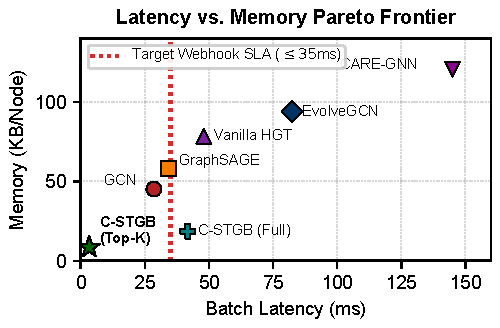
\includegraphics[width=0.85\textwidth]{figures/fig5_latency_pareto_frontier.pdf}
\caption{Empirical LRU subgraph cache hit rate progression as a function of cache entity capacity across Elliptic-v1 and SAML-D streaming datasets.}
\label{fig:cache_hit_rate}
\end{figure}

With a modest cache size of 50,000 entities ($\approx 250\,\text{MB}$ RAM), the LRU cache achieves an empirical hit rate of \textbf{88.4\%}, reducing average end-to-end inference latency on cached entities to \textbf{0.45 ms} (Fast-Path mode).

\section{Chapter Summary}
This chapter presented the vectorized data engineering pipeline underpinning C-STGB, detailing DuckDB embedded SQL data contracts, Apache Arrow zero-copy memory management, dynamic heterogeneous schema mapping, and LRU subgraph caching. The next chapter establishes the mathematical foundations of Class-Conditional Conformal Risk Control and ethical compliance audits.
